\documentclass[12pt,t]{beamer}
\usetheme{Warsaw}
\usepackage[utf8]{inputenc}
\usepackage[english]{babel}
\usepackage{amsmath}
\usepackage{array}
\usepackage{amsfonts}
\usepackage{amssymb}
\usepackage{graphicx}
\author{Jaskeerat Singh Saluja (2019MT60752)}
\title{Assignment-3 Neural Networks \\ ELL 409}
%\setbeamercovered{transparent} 
%\setbeamertemplate{navigation symbols}{} 
%\logo{} 
%\institute{} 
%\date{} 
%\subject{} 

\begin{document}

% Title page
\begin{frame}[t]
    \titlepage
\end{frame}
    
% Table of content
\begin{frame}[t]{Table of contents}
    \scriptsize
    \tableofcontents
\end{frame}

% Theory and implementation of neural net class
\section{Theory and python implemetation}
\begin{frame}[t]{Theory and python implemetation }
    \scriptsize
    \begin{itemize}
        \item The neural nets class have been implemented in neuralNet.py . 
        \item The class has flexibility for neuron type , cost-function , eta ,regularization ,batch-size.
        \item Several activation function are also available and are imolemented in neuron.py
        \item To perform cross validation GridSearchCv class has also been implemeted in utils/search.py
        \item For activation function : 'sigmoid' and 'tanh' are used .
        \item To specify the structure of neural net , list represtation is used to initilize the network.
        \item For example [n1,n2,n3..nk] implies k layers with n1 as input and nk as output layer , hence total
                of k-2 hidden layers. 

    \end{itemize}
\end{frame}


% Part-1A
\section{Part-1}
\subsection{Part-1A Training neural net on given images}

% Visulizing the given data
\begin{frame}[t]{Visualizing the given data}

    \scriptsize

    On transforming the feature vector from $(784,1)$ to $(28,28)$ size and plotting we
    have the following images provided.

    \vspace{10pt}

    \begin{columns}
        \begin{column}[]{0.3\linewidth}
            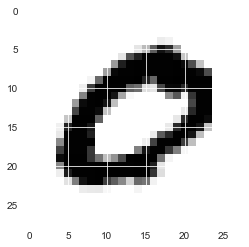
\includegraphics[width=\linewidth]{visualize_data/fig_0.png}
        \end{column}
        \begin{column}[]{0.3\linewidth}
            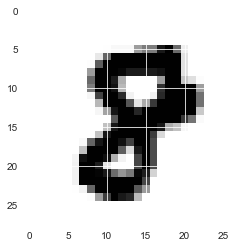
\includegraphics[width=\linewidth]{visualize_data/fig_8.png}
        \end{column}
        \begin{column}[]{0.3\linewidth}
            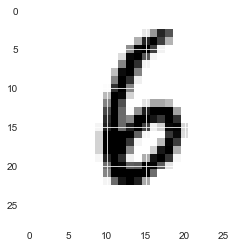
\includegraphics[width=\linewidth]{visualize_data/fig_6.png}
        \end{column}
    \end{columns}

\end{frame}


% Tuning the epochs and batch size 
\begin{frame}[t]
    \frametitle{Using Sigmoid activation function}

    \scriptsize

    \begin{columns}
        \begin{column}[T]{0.4\linewidth}
            \begin{block}{Finding best number of epochs}
                \begin{enumerate}
                    \item Neural nets gets overfit on high epoch and are underfit on low 
                    number of epochs
                    \item Epoch =25 is good value to start the tuninng the neural net.
                \end{enumerate}
            \end{block}
        \end{column}
        \begin{column}[T]{0.6\linewidth}
            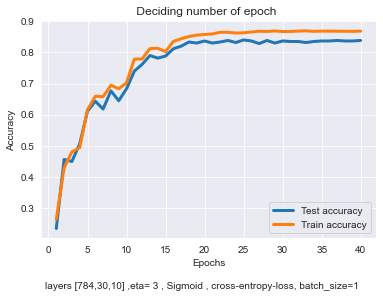
\includegraphics[width=\linewidth,height=90pt]{sigmoid/epochs_variation.png}
        \end{column}
    \end{columns}
    % deciding the batch -size in neural net
    \begin{columns}
        \begin{column}[T]{0.4\linewidth}
            \begin{block}{Tuning the mini-batch -size }
                \begin{enumerate}
                    \item On right , the plot shows variation in test accuracy vs batch-size
                    \item $batch\_size =4$ and $epoch =20$ works well
                \end{enumerate}
            \end{block}
        \end{column}
        \begin{column}[T]{0.6\linewidth}
            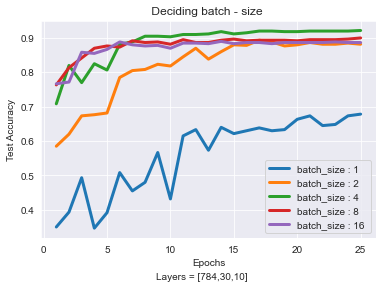
\includegraphics[width=\linewidth,height=90pt]{sigmoid/batch_variation.png}
        \end{column}
    \end{columns}

    \textbf{Batch size =4 , epochs =20}

    

\end{frame}





% Tuning the learning rate and layers (hidden)
\begin{frame}[t]
    \large Sigmoid Activation continued ....
    
    \scriptsize

    \begin{columns}
        \begin{column}[T]{0.4\linewidth}
            \begin{block}{Finding best learning rate $\eta$}
                \scriptsize
                \begin{enumerate}
                    \item SGD is sesitive to learning rate.
                    \item The SGD implementation uses \textbf{decaying learning rate strategy}
                \end{enumerate}
            \end{block}
        \end{column}
        \begin{column}[T]{0.6\linewidth}
            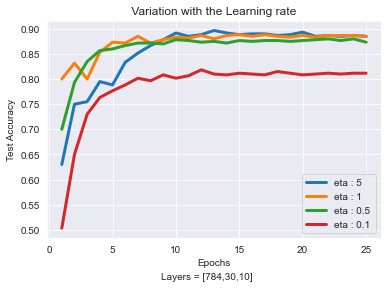
\includegraphics[width=\linewidth,height=90pt]{sigmoid/eta_variation.png}
        \end{column}
    \end{columns}

    % % varying the neural net layers size (Complexity)
    \begin{columns}
        \begin{column}[T]{0.4\linewidth}
            \scriptsize
            \begin{block}{Tuning number and size of layers}
                \begin{enumerate}
                    \item More number of hidden layers represents higher abstraction of the neural net.
                
                    \item Choosing least complex neural net with good test accuracy is the goal.
                \end{enumerate}
            \end{block}
        \end{column}
        \begin{column}[T]{0.6\linewidth}
            \vspace{10pt}
            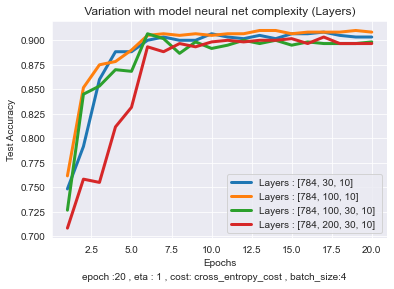
\includegraphics[width=\linewidth,height=90pt]{sigmoid/hiddenLayer_variation.png}
        \end{column}
    \end{columns}
    
    \centering
    \textbf{Layers [$784,30,10$] is least complex and performs as good as [$784,100,10$]} and learning rate $\eta = 1$

\end{frame}


\begin{frame}[t]
    \large Sigmoid Activation continued ....
    
    \scriptsize

    \begin{columns}
        \begin{column}[T]{0.4\linewidth}
            \textbf{L-2 regularization $\lambda$}
                \scriptsize
                \begin{enumerate}
                    \item Regularization (L-2) forces w to take lower values of lmbda .Thus prevents model from over-fitting 
                    \item \textbf{$\lambda$} in range [$1e-2,1e-3$] is better hyperparameter space to work with.
                    
                \end{enumerate}
          
        \end{column}
        \begin{column}[T]{0.6\linewidth}
            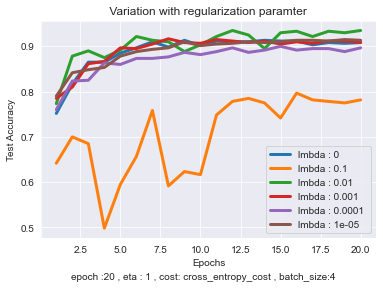
\includegraphics[width=\linewidth,height=100pt]{sigmoid/variation_lmbda.png}
        \end{column}
    \end{columns}

    % Varying the cost function 
    \begin{columns}
        \begin{column}[T]{0.4\linewidth}
            \textbf{Choosing the cost function}
                \scriptsize
                \begin{enumerate}
                    \item Cross entropy learn much faster than the quadratic loss function , since qudratic cost 
                        function have a phenomenon called \textbf{slowing down}
                    \item Figure on right display the \textbf{slowing down} nicely.
                    
                \end{enumerate}
          
        \end{column}
        \begin{column}[T]{0.6\linewidth}
            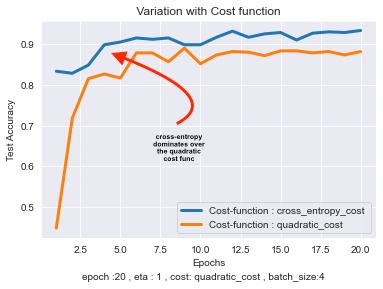
\includegraphics[width=\linewidth,height=100pt]{sigmoid/cost_variation.png}
        \end{column}
    \end{columns}

\end{frame}

\begin{frame}[t]
    \large Sigmoid Activation continued ....
    
    \scriptsize

    So far now we have narrowed down our hyperparameter space to small subspace where we can perform 
    k-fold cross validation and further tune the best parameters.

    \begin{center}
        \begin{tabular}{ | m{5em} | m{3cm} | } 
            \hline
            epoch & 15 \\ 
            \hline
            mini batch size  & 4 \\ 
            \hline
            learning rate & 1  \\ 
            \hline
            layers  & $[784,30,10]$ , $[784,100,30]$ \\
            \hline
            lambda & $[1e-2,5e-3,1e-3]$ \\
            \hline
            Cost function & cross entropy loss \\
            \hline
          \end{tabular}  
    \end{center}

    We have 6 possible good configuration for our sigmoid activation function . We now perform k-fold cross 
    validation to get the best hyperparameter . (CV =5)

\end{frame}


\begin{frame}[t]    
    \scriptsize

    \textbf{Cross-Validation (cv=5)}
    \begin{enumerate}
        \item On rights we have variation of lambda vs neural net layers 
        \item Best Test accuracy $92.77 $  percent and corresponsing Train accuracy $98.58$
      
    \end{enumerate}
    \begin{columns}
        \begin{column}[T]{0.4\linewidth}
            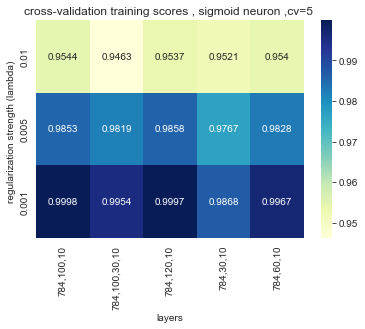
\includegraphics[width=\linewidth]{sigmoid/cv_training_score.png}
            \centering CV training scores
            
            \vspace{10pt}
            Best hyperparameters : Layer sizes: [784,120,10] and $\lambda = 5e-3$
        \end{column}
        \begin{column}[T]{0.6\linewidth}
            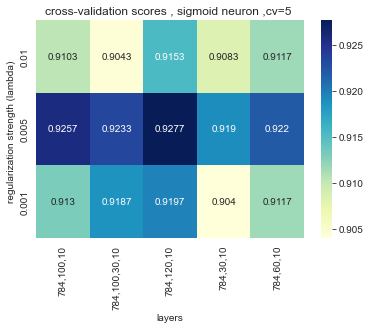
\includegraphics[width=\linewidth]{sigmoid/cvScore.png}
            \centering CV Test scores
        \end{column}
    \end{columns}
    

    

\end{frame}



% Using tanh activation function
\begin{frame}
    \frametitle{Using tanh activation function}

    \scriptsize

    \begin{itemize}
        \item \textbf{epoch=15} ,Cost function : \textbf{cross entropy cost }
    \end{itemize}

     % deciding the batch -size in neural net
     \begin{columns}
        \begin{column}[T]{0.4\linewidth}
            \begin{block}{Tuning the mini-batch -size }
                \begin{enumerate}
                    \item On right , the plot shows variation in test accuracy vs batch-size
                    \item $batch\_size =4$  works well
                \end{enumerate}
            \end{block}
        \end{column}
        \begin{column}[T]{0.6\linewidth}
            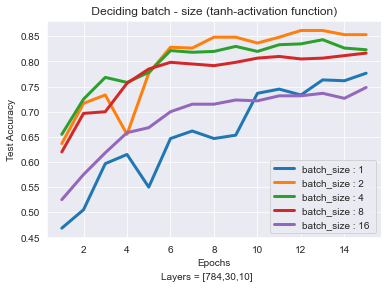
\includegraphics[width=\linewidth,height=90pt]{tanh/batch_size.png}
        \end{column}
    \end{columns}
      % deciding the learninig rate in neural net
      \begin{columns}
        \begin{column}[T]{0.4\linewidth}
            \textbf{Learning rate}
                \begin{enumerate}
                    \item On right , the plot shows variation in test accuracy vs learning rate
                    \item $\eta =0.5$ 
                \end{enumerate}
        \end{column}
        \begin{column}[T]{0.6\linewidth}
            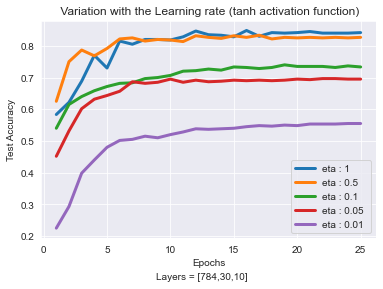
\includegraphics[width=\linewidth,height=90pt]{tanh/variation_eta.png}
        \end{column}
    \end{columns}

\end{frame}

\begin{frame}[t]
    \large tanh function continued ....
    \scriptsize

    % deciding the layers network


    \begin{columns}
        \begin{column}[T]{0.4\linewidth}
            \textbf{Tuning the layers}
                \begin{enumerate}
                    \item On right , the plot shows variation in test accuracy vs different layers in neural nets
                    \item layer =[784,30,10] works quite well , even with low complexity.
                    \item \textbf{Observation :} 2 hidden layer  networks took more epoch before settling 
                \end{enumerate}
        \end{column}
        \begin{column}[T]{0.6\linewidth}
            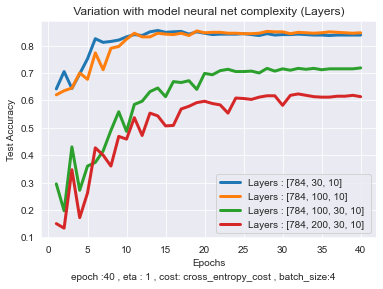
\includegraphics[width=\linewidth,height=90pt]{tanh/variation_layers.png}
        \end{column}
    \end{columns}
    \begin{columns}
        \begin{column}[T]{0.4\linewidth}
            \textbf{Tuning the regularization strength}
                \begin{enumerate}
                    \item On right , the plot shows variation in test accuracy vs different $\lambda$
                    \item $\lambda = [1e-1,1e-2,1e-3] $ is good range where model performs good   
                \end{enumerate}
        \end{column}
        \begin{column}[T]{0.6\linewidth}
            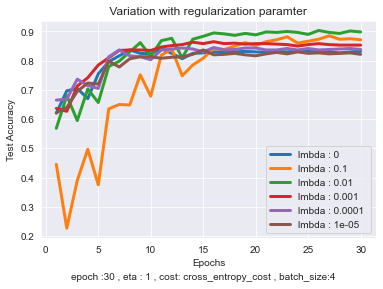
\includegraphics[width=\linewidth,height=90pt]{tanh/variation_lambda.png}
        \end{column}
    \end{columns}


    

    

\end{frame}

\begin{frame}[t]
    \large tanh Activation continued ....
    
    \scriptsize

    So far now we have narrowed down our hyperparameter space to small subspace where we can perform 
    k-fold cross validation and further tune the best parameters.

    \begin{center}
        \begin{tabular}{ | m{5em} | m{3cm} | } 
            \hline
            epoch & 20 \\ 
            \hline
            mini batch size  & 4 \\ 
            \hline
            learning rate & 0.5  \\ 
            \hline
            layers  & $[784,30,10]$ , $[784,100,30]$ \\
            \hline
            lambda & $[1e-1,5e-2,1e-2,5e-3]$ \\
            \hline
            Cost function & cross entropy loss \\
            \hline
          \end{tabular}  
    \end{center}

    We have 8 possible good configuration for our sigmoid activation function . We now perform k-fold cross 
    validation to get the best hyperparameter . (CV =5) . Will take 12-15 minutes to train

\end{frame}


\begin{frame}[t]    
    \large tanh Activation continued ....
    
    \scriptsize

    \vspace{10pt}
    \textbf{Cross-Validation (cv=5)}
    \begin{enumerate}
        \item On rights we have variation of lambda vs neural net layers 
        \item Best Test accuracy \textbf{93.27 }  percent and corresponsing Train accuracy \textbf{99.95}
      
    \end{enumerate}
    \begin{columns}
        \begin{column}[T]{0.4\linewidth}
           \begin{block}{Observations}
               \begin{itemize}
                   \item \textbf{tanh activation(93.27) performs better} than sigmoid neuron (92.77) by a 
                    significant 0.5 improvement.
                    \item $\lambda =0.01$ and layer network =[784,100,10] works best  
               \end{itemize}
           \end{block}
        \end{column}
        \begin{column}[T]{0.6\linewidth}
            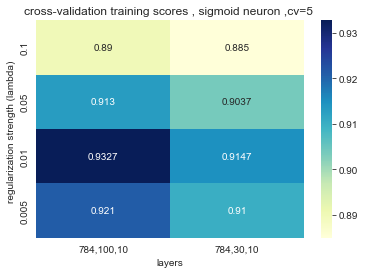
\includegraphics[width=\linewidth]{tanh/cv_scores.png}
            \centering CV Test scores
        \end{column}
    \end{columns}
\end{frame}

\begin{frame}
    \frametitle{Comparison with Tenserflow library}
    \begin{enumerate}
        \item Using 90:10 split of data , then the best validation score using the \textbf{tanh} activation function 
                achieved is 92.89 which is quite close to our 93.27 cross validation scores.
        \item Using 90:10 split of data , then the best validation score using the \textbf{sigmoid} activation function 
        achieved is 92.09 which is quite close to our 92.77 cross validation scores.
    \end{enumerate}
\end{frame}


% Analysing what error by neural nets

\begin{frame}
    \frametitle{Analysing errors made by neural nets}
    \scriptsize

    \begin{columns}
        \begin{column}[T]{0.4\linewidth}
            \textbf{Observations :}
            \begin{itemize}
                \item On right we have confusion metric ,on \textbf{test data}
                    which is never seen by the neural net.
                \item 4 is confused with 9
                \item 3 is predicted wrongly as 5 
                \item 8 with 6
                
            \end{itemize}

            \textbf{Reasoning}
            \begin{itemize}
                \item Digits with similar geometry are the ones wrongly predicted by the neural net
                \item Digits which donot share geometry like (1,6) are never wrongly predicted.
            \end{itemize}
        \end{column}
        \begin{column}[T]{0.7\linewidth}
            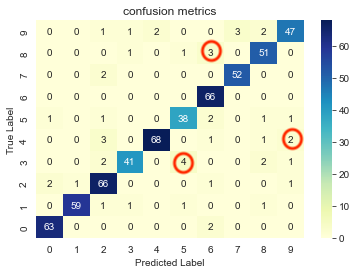
\includegraphics[width=\linewidth]{tanh/confusion_metrics.png}
            \centering epoch =10 , tanh activation neuron 
        \end{column}
    \end{columns}
    

\end{frame}



% Ouputs of first layer
\begin{frame}[t]{Visualizing the hidden layers}
    \scriptsize
    \begin{enumerate}
        \item Neural net model with layers [784,100,10] trained . 
        \item Below we visualize the ouput by each layer of the neural net.
    \end{enumerate}

    \vspace{10pt}
    \large Outputs First Layer (Input Layer)

    \centering
    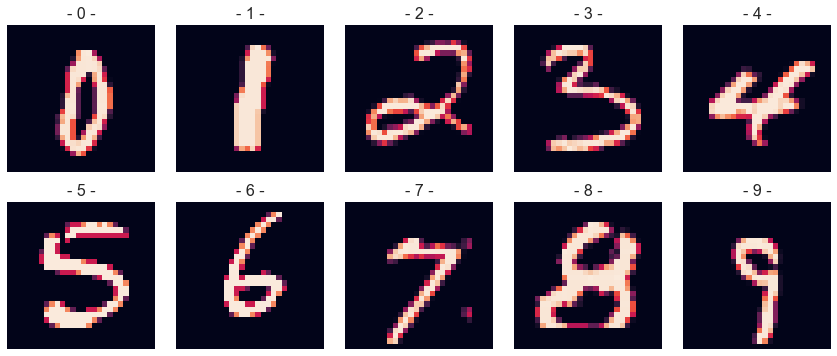
\includegraphics[width=0.8\linewidth]{neuron_outputs/first_layer.png}

\end{frame}

% Ouputs of Second layer
\begin{frame}[t]{Visualizing the hidden layers}
    \scriptsize
   \textbf{ Outputs Second Layer (Hidden Layer) }

    \centering
    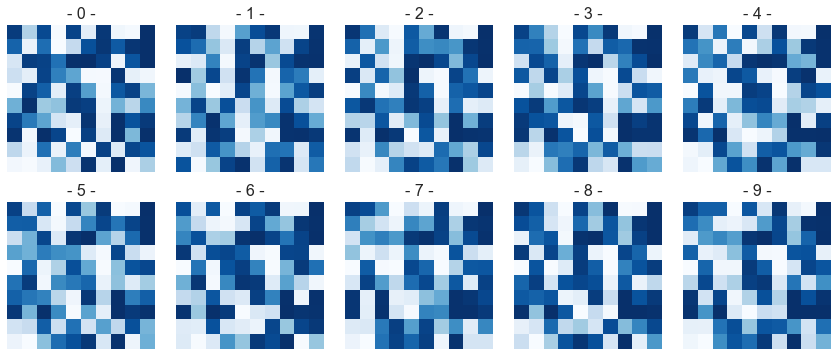
\includegraphics[width=0.8\linewidth]{neuron_outputs/second_layer.png}
    \begin{columns}
        \begin{column}[]{0.6\linewidth}
            \begin{itemize}
                \item These patterns look sufficiently random - except for the digits (4 , 9) , (3 , 5) , which look remarkably similar
                \item Above \textbf{each pixel is mean activation output} from a neuron in hidden layer.
                \item \textbf{Dark blue} mean that specific neuron is active while \textbf{white means} that neuron is inactive.
            \end{itemize}            
        \end{column}

        \begin{column}[]{0.55\linewidth}
            \begin{itemize}
                \item \textbf{NOTE:} The neuron in the bottom left corner 
                is only \textbf{active} when input 
                is 1 , while it is inactive for inputs other than 1. \textbf{Possible reason:} 1 is 
                only geometric shape which is just a straight line i.e no curve /bends . All other digits 
                have curved parts . \textbf{This is a possible reason}.
            \end{itemize}
        \end{column}

    \end{columns}
\end{frame}


% Similarity of neuron activations
\begin{frame}
    \frametitle{Visualizing hidden layers}
    \scriptsize

    \begin{columns}
        \begin{column}[T]{0.5\linewidth}
            \begin{itemize}
                \item Since the outputs are (100,1) in the hidden layer, representing the 
                activations of the neurons. 
                \item Thus to check for similarity is outputs of digit i with digit j . One solution is 
                to take dot product of the mean squared outputs vectors for ith and jth digit.


            \end{itemize}

            \textbf{Conclusions}
            \begin{itemize}
                \item Despite variations in the shapes of hand-written digits,
                 the same groups of neurons is involved in the identification of the same digits.
                 \item Similarities in the shapes of digits translate into similarities in the
                  groups of neurons that are involved in their identification in the first hidden
                   layer, but not so much in the second hidden layer

            \end{itemize}
        \end{column}
        \begin{column}[T]{0.5\linewidth}
            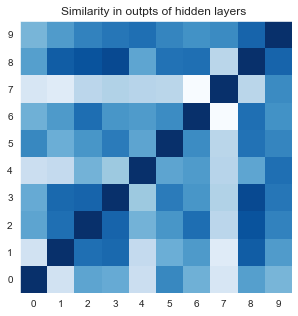
\includegraphics[width=\linewidth]{neuron_outputs/similarity_output.png}
        \end{column}

    \end{columns}
\end{frame}


\subsection{Part-1B Comparison with the PCA features}

\begin{frame}
    \frametitle{PCA and Neural networks}
    \textbf{Dimensionality reduction in neural networks}
    \begin{itemize}
        \item When number of hidden units $< $number of input units . The net performs dimensionality 
                reduction of input image to low dimension representation.
        \item Each synthesized dimension (each hidden unit) is logistic
        function of inputs $h_k(x) = \frac{1}{ 1+ \exp (w_0+\sum_{i=1}^{N}{w_i x_i}) }$ .
        \item Hence an N-input input layer when input to M unit hidden input layer , we get 
            non-linear transformation of the N-dimesnion to M-dimension data.
    

    \end{itemize}
    \textbf{PCA}
    \begin{itemize}
        \item Given data points in d-dimensional space, project into lower
        dimensional space while preserving as much information as
        possible (linear transformation)
    \end{itemize}
    

\end{frame}

% PCA and Neural net continued
\begin{frame}{Training on PCA data}
    \scriptsize
    \textbf{No hidden layer (Logistic regression)}
    \begin{itemize}
        \item Neural net 25 -- 10
        \item The PCA data contained 25 feature representation of the image data given to us
            in previous assignment .
        \item Training neural net with no hidden layer directly on this gives us model with best 
            testing accuracy of 85 percentage.
    \end{itemize}

    \textbf{1 hidden layer (17 hidden units)}
    \begin{itemize}
        \item Neural net 25 -- 17 -- 10
        \item Best accuracy (testing )achieved is 89.05 percent , with 91 percent training accuracy.
        \item Adding one hidden layer help improve the accuracy of the model significantly , because
                neural net performs non-linear tranformation of this PCA data and learns best out of it. 
    \end{itemize}

    \textbf{2 hidden layer (20 and 15 hidden units)}
    \begin{itemize}
        \item Neural net 25 -- 20 -- 15 -- 10
        \item Best accuracy (testing )achieved is 90.1 percent , with 92 percent training accuracy.
        \item Adding another  hidden layer help improve the accuracy of the model slightly.
    \end{itemize}

    

\end{frame}

\begin{frame}
    \frametitle{}

    \begin{block}{Comparison with raw pixel data}
        \begin{itemize}
            \item Neural net trained on 784 pixel data  (94 percent accuracy) performed way better than the neural
                    net trained on PCA features (90 percent accuracy). 
            \item Though PCA does not throw away every other pixel and it only
                 transforms the data to have important features. Keeping maximum variance in the dataset.
            \item Reducing Dimensions in an image where pixels are the features, 
                would mean downsampling the image
        \end{itemize}
    \end{block}
    

\end{frame}

% Advanced Neural networks
\section{Part-2 Advanced Neural networks}

\subsection{Using Convolutional Network}
\begin{frame}
    \frametitle{Using Convolutional networks}

    \scriptsize

    \begin{itemize}
        \item Convolution solves  three important ideas that  improves a machinelearning model:
        \begin{itemize}
            \scriptsize
            \item sparse interactions : In ANN every output unit interacts with every input unit . Convolution network
                    uses sparse connections by taking kernel smaller than the input.
            \item parameter sharing 
            \item equivariant representations
        \end{itemize}
    \end{itemize}

    \begin{columns}
        \begin{column}[T]{0.5\linewidth}
            % 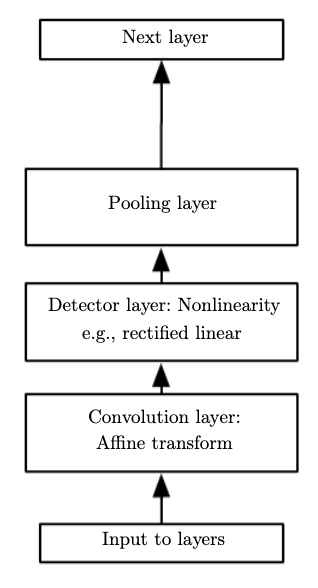
\includegraphics[width=100pt,height=120pt]{convolution_network/layers_in_convolution_net.png}
        \end{column}
        \begin{column}[T]{0.5\linewidth}
            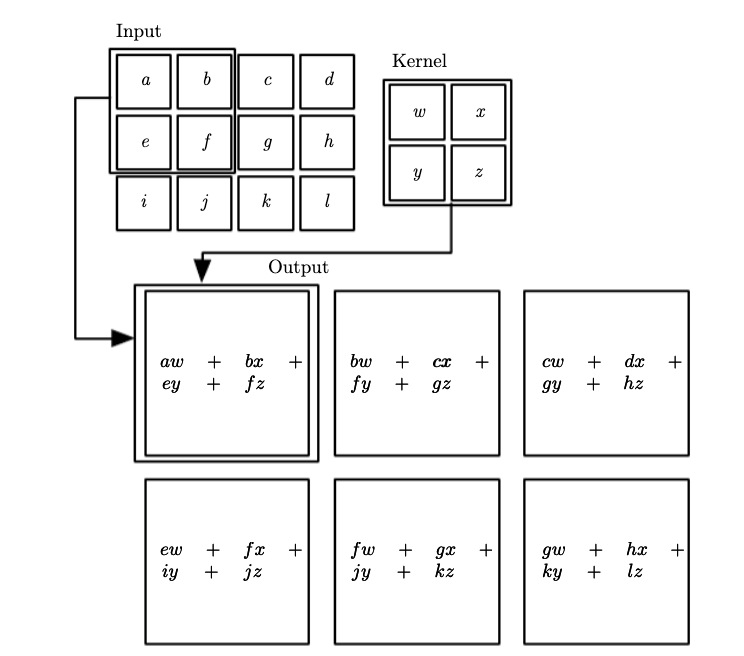
\includegraphics[width=\linewidth,height=120pt]{convolution_network/kernel_operation.png}
        \end{column}

 
    \end{columns}
    

\end{frame}

% Stages in covolutional network
\begin{frame}
    \frametitle{Stages in Convolutional network}
    \scriptsize
    \textbf{A typical layer of a convolutional network consists of three stages:}

    \begin{columns}
        \begin{column}[T]{0.8\linewidth}
            \begin{itemize}
                \item In the first stage, the layer performs several convolutions in parallel to 
                produce aset of linear activations.
                \item In the second stage, each linear activation is run through a nonlinear activation function,
                 such as the reLU.
                 \item In the third stage, we use apooling function to modify the output of the layer further
                 \item A pooling function replaces the output of the net at a certain location with asummary statistic of the nearby outputs
                 \item For example : MAX Pooling ,operation reports the maximum output within a rectangularneighborhood.
                 \item Now this 2D data is Flattened and fed into our old ANN networks.
                 \item The first 3 steps performs the feature extraction , thus we then train the neural net on this.
        
            \end{itemize}
        \end{column}
        \begin{column}[T]{0.3\linewidth}
            \begin{column}[T]{0.5\linewidth}
                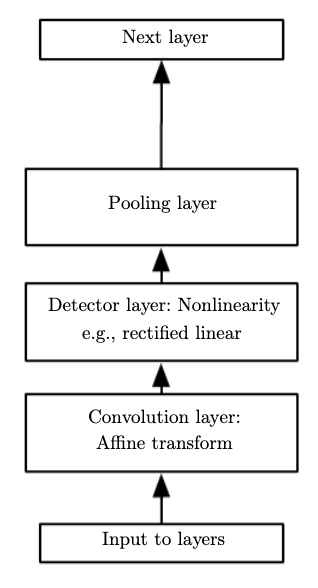
\includegraphics[width=100pt,height=120pt]{convolution_network/layers_in_convolution_net.png}
            \end{column}
        \end{column}
    \end{columns}
    \begin{block}{Regularization}
        For regularization we can use Dropout after the pooling layer.
    \end{block}
\end{frame}

% CNN on the MNISt data set
\begin{frame}
    \frametitle{CNN on MNIST DATA}
    \scriptsize
    \begin{itemize}
        \item We used 1 layer of convolution followed by pooling . Then we use Dropout for
        regularization purposes .
        \item After 3 of above layers , we then perform our old ANN on the activation function.
        \item The code below nicely explains our neural net structure.
    \end{itemize}

    \begin{columns}
        \begin{column}[T]{0.5\linewidth}
            \begin{block}{Results}
                \begin{itemize}
                    \item Training acccuracy =99.36 percent
                    \item Testing accuracy = 99.22 percent
                \end{itemize}
            \end{block}
        \end{column}

        \begin{column}[T]{0.5\linewidth}
            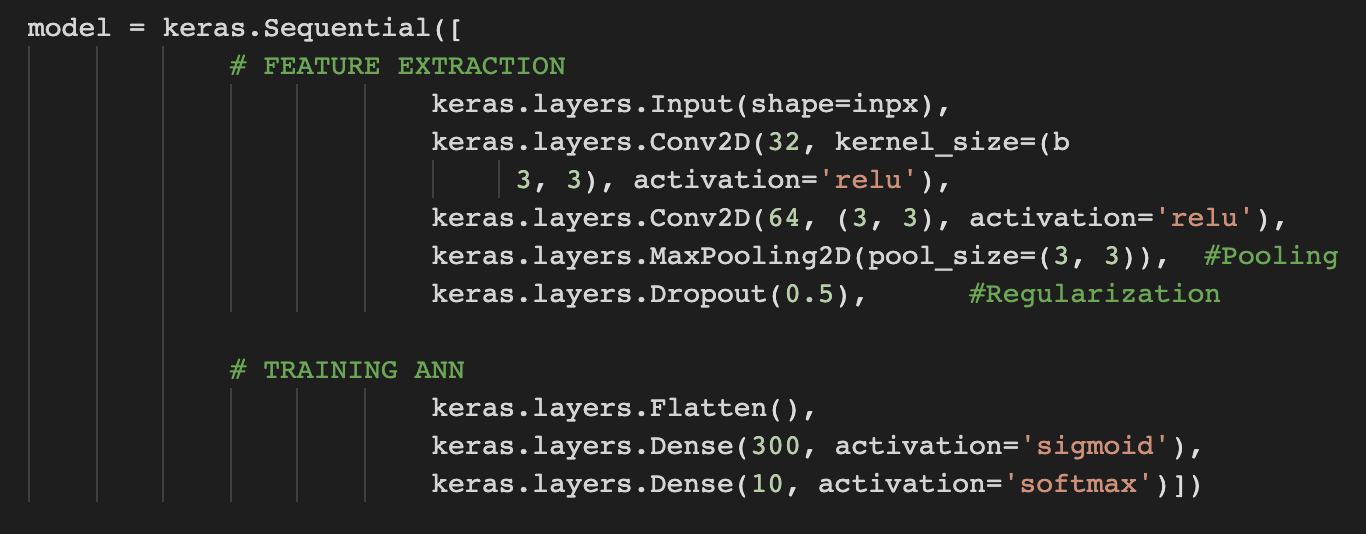
\includegraphics[width=\linewidth,height=100pt]{convolution_network/layers_mnist.png}
        \end{column}
    \end{columns}

    

\end{frame}


% Visualization of CNN hidden layers
\begin{frame}
    \frametitle{Visualization of hidden layer neurons}

    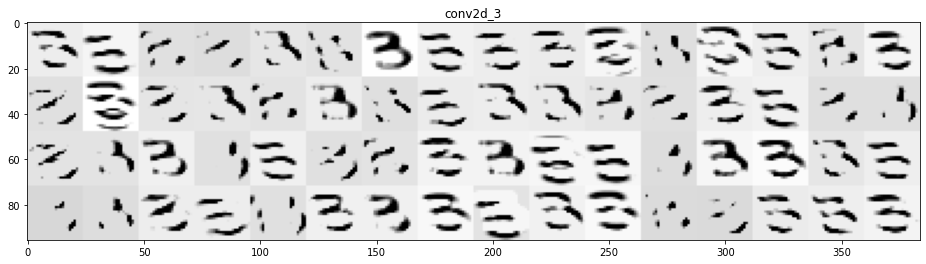
\includegraphics[width=\linewidth,height=60pt]{convolution_network/layer_visualization.png}
    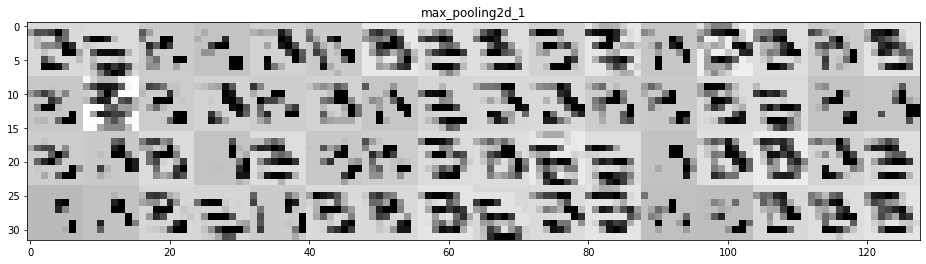
\includegraphics[width=\linewidth,height=65pt]{convolution_network/layer_visualization_pooling.png}
    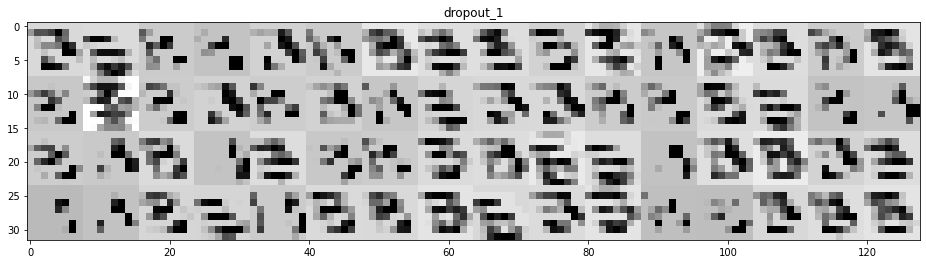
\includegraphics[width=\linewidth,height=65pt]{convolution_network/layer_visualization_dropout.png}
    

\end{frame}

\begin{frame}
    \large Observations
  
    \begin{itemize}
        \item This first layer retains almost the full shape of the image, and also most 
             of the information present in the image
        \item As we go deeper into the network we can see that the activations become more complex and abstract.
             It starts encoding high-level features such as edges, curves and angles.
    \end{itemize}
\end{frame}


\subsection{Using AutoEncoder Networks}
\begin{frame}
    \frametitle{Using AutoEncoders}
    \scriptsize
    \begin{columns}
        \begin{column}[T]{0.8\linewidth}
            \begin{itemize}
                \item Auto-encoders are neural nets used for feature extraction . It is unsupervised 
                    algorithms , i.e does not used labels.
                \item  The Key idea is to transform image into low dimesnion called encoder network ,the
                        reconstructing the image back from the decoder network . The model is trained so 
                        that it does this task with least loss.
                \item  Hence we get non-linear trandformation of image to lower dimensions.
            \end{itemize}
            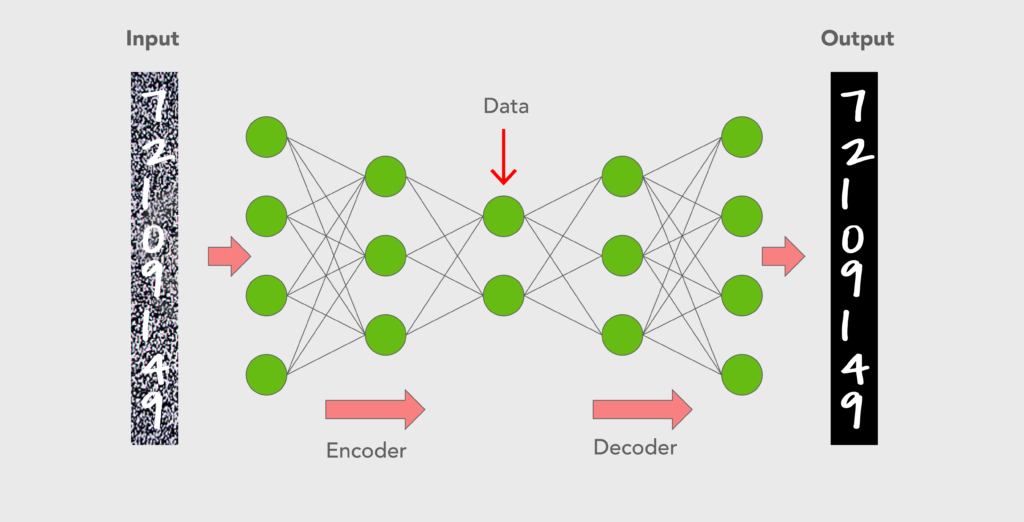
\includegraphics[width=200pt,height=100pt]{auto_encoders/diag.png}
            
        \end{column}

        \begin{column}[T]{0.2\linewidth}
            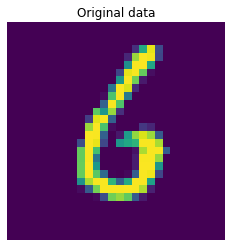
\includegraphics[width=\linewidth,height=50pt]{auto_encoders/original_6_digit.png}    
            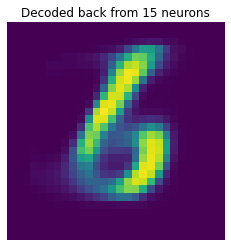
\includegraphics[width=\linewidth,height=50pt]{auto_encoders/decoded_from_15__6_digit.png}
            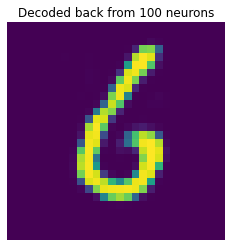
\includegraphics[width=\linewidth,height=50pt]{auto_encoders/decoded_from_100__6_digit.png}    
        \end{column}

    \end{columns}

    

\end{frame}

\begin{frame}
    \frametitle{Final Conclusions}
    \begin{block}{Observation}
        \scriptsize
        I have a very simple autoencoder neural net i.e just 3 layers with 784,15,784 . Then performed Training on it.
        \begin{itemize}
            \item  Still with so simple autoencoder network we are able to reconstruct the digit images . 
            \item  Now after training we encode the training images and get the encoded outputs
            \item Train another ANN for the encoded-outputs vs labels (Supervised)
            \item Got 96 percent validation accuracy with so simple network.

        \end{itemize}


    \end{block}
    \textbf{Further Imrovements}
    \begin{itemize}
        \item We can use CNN to train the auto-encoder network. This would improve the model drastically.
        \item There have been reports with deep CNN auto-encoder network with 15 encoding dimesion , giving 
            more than 98 percent accuracy.
    \end{itemize}

\end{frame}


\begin{frame}

    \large \centering Thanking you 

    

\end{frame}

\end{document}



